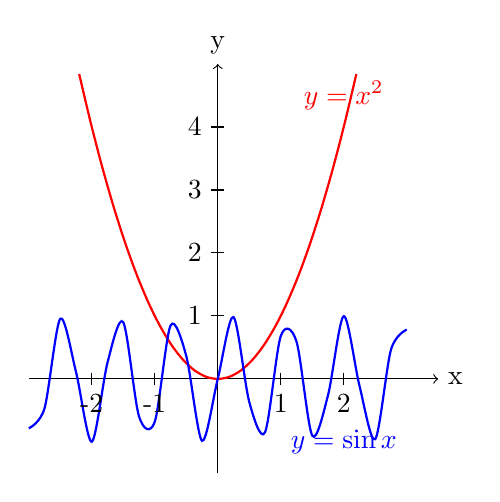
\begin{tikzpicture}[scale=0.8]
  \draw[->] (-3,0) -- (3.5,0) node[right] {x};
  \draw[->] (0,-1.5) -- (0,5) node[above] {y};
  \draw[scale=1,domain=-2.2:2.2,smooth,variable=\x,red,thick] plot ({\x},{\x*\x});
  \draw[scale=1,domain=-3:3,smooth,variable=\x,blue,thick] plot ({\x},{sin(\x r*180/3.14159)});
  \node[red] at (2,4.5) {$y=x^2$};
  \node[blue] at (2,-1) {$y=\sin x$};
  \foreach \x in {-2,-1,1,2} {\draw (\x,0.1) -- (\x,-0.1) node[below] {\x};}
  \foreach \y in {1,2,3,4} {\draw (0.1,\y) -- (-0.1,\y) node[left] {\y};}
\end{tikzpicture}